\documentclass[12pt,oneside,english]{amsart}
\usepackage[T1]{fontenc}
\usepackage{geometry}
\usepackage{parskip}
\geometry{verbose,tmargin=0.75in,bmargin=0.75in,lmargin=0.75in,rmargin=0.75in,headheight=0.75cm,headsep=1cm,footskip=1cm}
\setlength{\parskip}{\medskipamount}
\usepackage{setspace}
\onehalfspacing
\usepackage{multicol}
\usepackage{graphicx}
\usepackage{ulem}
\usepackage[export]{adjustbox}
\usepackage{enumitem}
\setlist[enumerate,1]{label=\textbf{\arabic*.}}
\makeatother
\usepackage{babel}
\usepackage{tikz, pgfplots}
\usepgfplotslibrary{polar}
\usepgfplotslibrary{fillbetween}
\usepackage{mathtools}
\usepackage{cancel}
\setlist[enumerate]{topsep=0.4cm}

\usepackage{fancyhdr}
\pagestyle{fancy}
\fancyhf{}
\rfoot{\copyright2020 Adam D. Richardson}
\renewcommand{\headrulewidth}{0pt}

\DeclarePairedDelimiter{\abs}{\lvert}{\rvert}


\begin{document}

\title{MATH 70 - Activity \#18 - Polar Coordinates Solutions}

\maketitle
\thispagestyle{empty}

%\vspace*{-5mm}
%\parbox[c]{\textwidth}{
%\hrule
%\vspace{3mm}
%Write your names and section number in the upper right hand corner of this page. Remember you will be graded on the accuracy, quality, clarity, and legibility of your work. Explanation and justification for your conclusions are more important than ``final answer''. Use complete sentences when appropriate.
%\vspace{3mm}
%\hrule}

\hrule \kern 1mm \hrule

\vspace{1cm}


\begin{enumerate}[leftmargin=*]
\setlength\itemsep{1.5cm}

\item First, plot the following point given in polar coordinates, then find two other equivalent pairs of polar coordinates of this point, one with $r>0$ and one with $r<0$. Second, find the Cartesian representation of these points.

\begin{enumerate}
\item $\left(1,\frac{\pi}{4}\right)$

\begin{center}
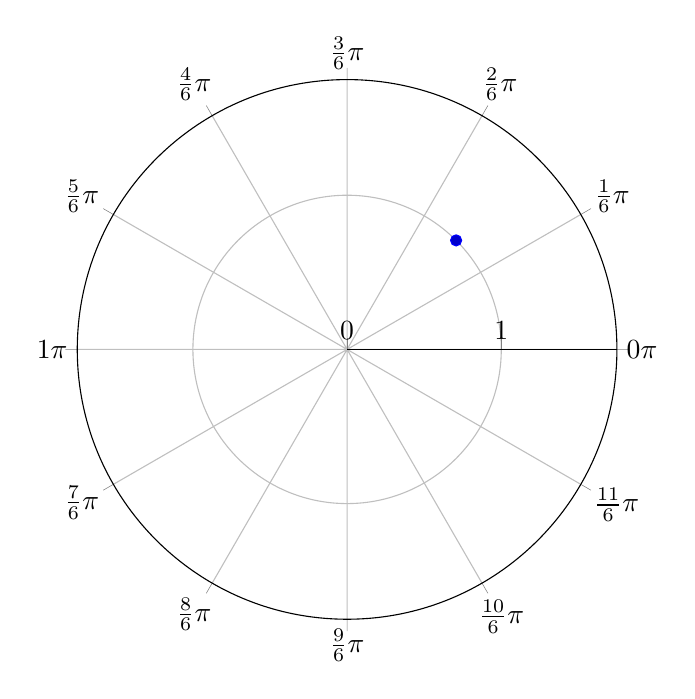
\begin{tikzpicture}
\begin{polaraxis}[
   xticklabel=$\pgfmathprintnumber{\tick}^\circ$,
   xtick={0,30,...,330},
   ytick={0,1},
   ymin=0, ymax=1.75,
   xticklabel={
\pgfmathparse{\tick/180}
\pgfmathifisint{\pgfmathresult}{$\pgfmathprintnumber[int detect]{\pgfmathresult}\pi$}%
{$\pgfmathprintnumber[frac,frac denom=6,frac whole=false]{\pgfmathresult}\pi$}
}
]

\addplot coordinates {(45,1)};
\end{polaraxis}
\end{tikzpicture}
\end{center}

By adding $2\pi$ to $\frac{\pi}{4}$, we get the equivalent point $\left(1,\frac{9\pi}{4}\right)$ and $r>0$. The direction opposite $\frac{\pi}{4}$ is $\frac{5\pi}{4}$, so we can get an equivalent point by negating the given radius: $\left(-1,\frac{5\pi}{4}\right)$.

To convert to Cartesian coordinates, we use the conversion equations $x=r\cos\theta$, $y=r\sin\theta$. Thus,

\[
x=1\cdot\sin\frac{\pi}{4}=\frac{\sqrt{2}}{2}\hspace{0.5cm}\text{and}\hspace{0.5cm}y=1\cdot\sin\frac{\pi}{4}=\frac{\sqrt{2}}{2},
\]

so our point is $\left(\frac{\sqrt{2}}{2},\frac{\sqrt{2}}{2}\right)$. Notice this agrees with our sketch.

\item $\left(-2,\frac{3\pi}{2}\right)$

\begin{center}
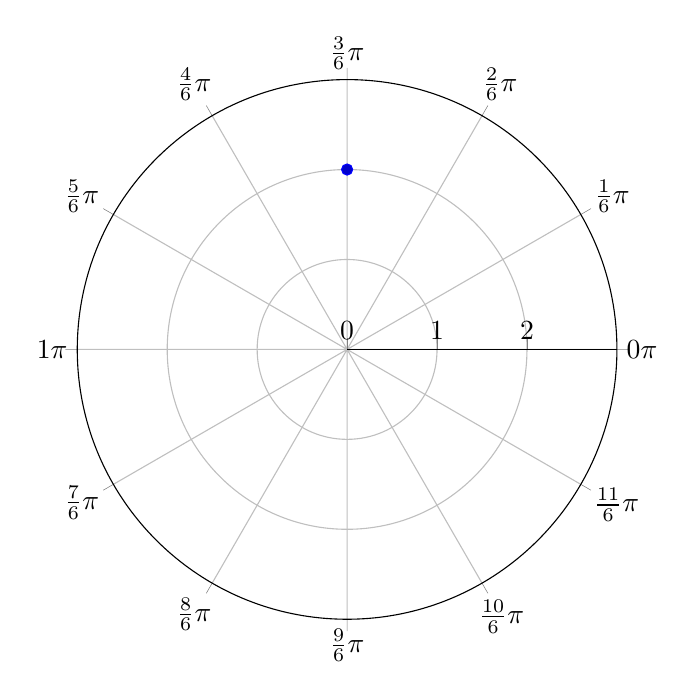
\begin{tikzpicture}
\begin{polaraxis}[
   xticklabel=$\pgfmathprintnumber{\tick}^\circ$,
   xtick={0,30,...,330},
   ytick={0,1,2},
   ymin=0, ymax=3,
   xticklabel={
\pgfmathparse{\tick/180}
\pgfmathifisint{\pgfmathresult}{$\pgfmathprintnumber[int detect]{\pgfmathresult}\pi$}%
{$\pgfmathprintnumber[frac,frac denom=6,frac whole=false]{\pgfmathresult}\pi$}
}
]

\addplot coordinates {(270,-2)};
\end{polaraxis}
\end{tikzpicture}
\end{center}

$\left(-(-2),\frac{3\pi}{2}-\pi\right)=\left(2,\frac{\pi}{2}\right)$, and $\left(-2,\frac{3\pi}{2}+2\pi\right)=\left(-2,\frac{7\pi}{2}\right)$.

\[
x=-2\cos\frac{3\pi}{2}=0\hspace{0.5cm}\text{and}\hspace{0.5cm}y=-2\sin\frac{3\pi}{2}=2,
\]

so the point is $(0,2)$. Notice this agrees with our sketch.
\end{enumerate}


\item Sketch the following region in the plane: $2<r<3$, \hspace{0.25cm}$\frac{5\pi}{3}\leq\theta\leq\frac{7\pi}{3}$

\begin{center}
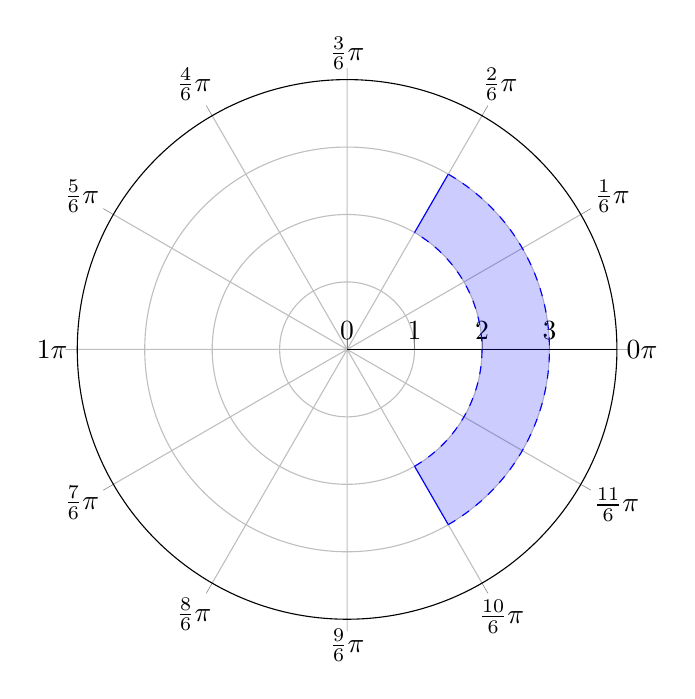
\begin{tikzpicture}
\begin{polaraxis}[
   xticklabel=$\pgfmathprintnumber{\tick}^\circ$,
   xtick={0,30,...,330},
   ytick={0,1,2,3},
   ymin=0, ymax=4,
   xticklabel={
\pgfmathparse{\tick/180}
\pgfmathifisint{\pgfmathresult}{$\pgfmathprintnumber[int detect]{\pgfmathresult}\pi$}%
{$\pgfmathprintnumber[frac,frac denom=6,frac whole=false]{\pgfmathresult}\pi$}
}
]

\addplot[name path=A, domain=300:420, samples=100, style=dashed, color=blue] (x,2);
\addplot[name path=B, domain=300:420, samples=100, style=dashed, color=blue] (x,3);
\tikzfillbetween[of=A and B]{blue, opacity=0.2};
\addplot[mark=none, color=blue] coordinates {(300,2) (300,3)};
\addplot[mark=none, color=blue] coordinates {(420,2) (420,3)};
\end{polaraxis}
\end{tikzpicture}
\end{center}

\item Sketch the following curves by first sketching the graph of $r$ as a function of $\theta$ in Cartesian coordinates.

\begin{enumerate}
\item $r=1+2\cos\theta$

\begin{multicols}{2}
\begin{center}
\begin{tikzpicture}[scale=1]
\begin{axis}[
	axis lines=middle,
	xmin=0, xmax=6.8,
	ymin=-2.25, ymax=4.5,
	xtick={1.570796327,	3.141592654,	4.71238898,	6.283185307},
	ytick={-2,...,4},
	xticklabels={$\frac{\pi}{2}$, $\pi$, $\frac{3\pi}{2}$, $2\pi$},
	axis line style={->},
	%grid=both,
	ticklabel style={font=\tiny,fill=white},
	xlabel=$\theta$, ylabel=$r$,
	xlabel style={at={(ticklabel* cs:1)},anchor=north west},
	ylabel style={at={(ticklabel* cs:1)},anchor=south west}
]

\addplot[thick, samples=100, domain=0:2*pi] {1+2*cos(deg(x))};

\end{axis}
\end{tikzpicture}
\end{center}

\columnbreak

\begin{center}
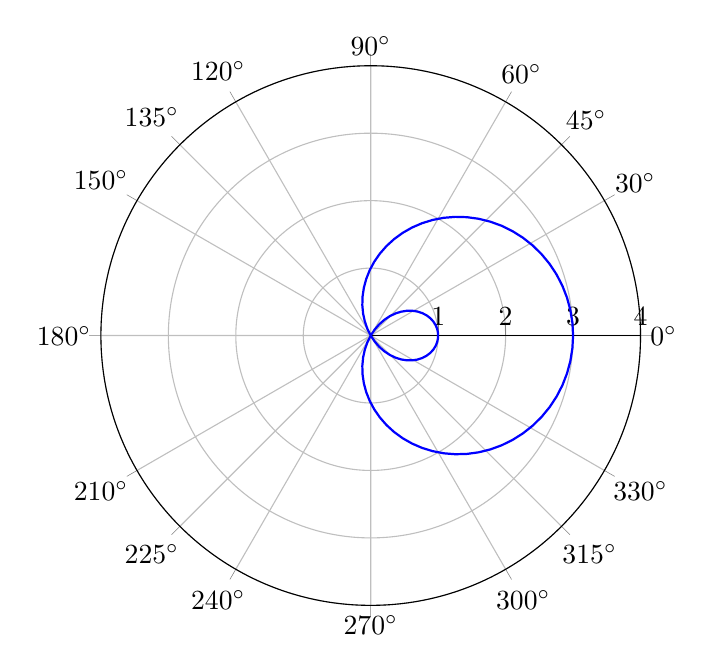
\begin{tikzpicture}
\begin{polaraxis}[
   xticklabel=$\pgfmathprintnumber{\tick}^\circ$,
   xtick={0,30,45,60,90,120,135,150,180,210,225,240,270,300,315,330},
   ytick={1,2,3,4},
  % yticklabel={1,2,3};
   ymin=0, ymax=4];
   
\addplot[thick, color=blue, domain=0:360, samples=100] {1+2*cos(x)};  
   

\end{polaraxis}
\end{tikzpicture}
\end{center}

\end{multicols}



\item $r=3\cos\theta$

\begin{multicols}{2}
\begin{center}
\begin{tikzpicture}[scale=1]
\begin{axis}[
	axis lines=middle,
	xmin=0, xmax=6.8,
	ymin=-3.25, ymax=3.5,
	xtick={1.570796327,	3.141592654,	4.71238898,	6.283185307},
	ytick={-3,...,3},
	xticklabels={$\frac{\pi}{2}$, $\pi$, $\frac{3\pi}{2}$, $2\pi$},
	axis line style={->},
	%grid=both,
	ticklabel style={font=\tiny,fill=white},
	xlabel=$\theta$, ylabel=$r$,
	xlabel style={at={(ticklabel* cs:1)},anchor=north west},
	ylabel style={at={(ticklabel* cs:1)},anchor=south west}
]

\addplot[thick, samples=100, domain=0:2*pi] {3*cos(deg(x))};

\end{axis}
\end{tikzpicture}
\end{center}

\columnbreak

\begin{center}
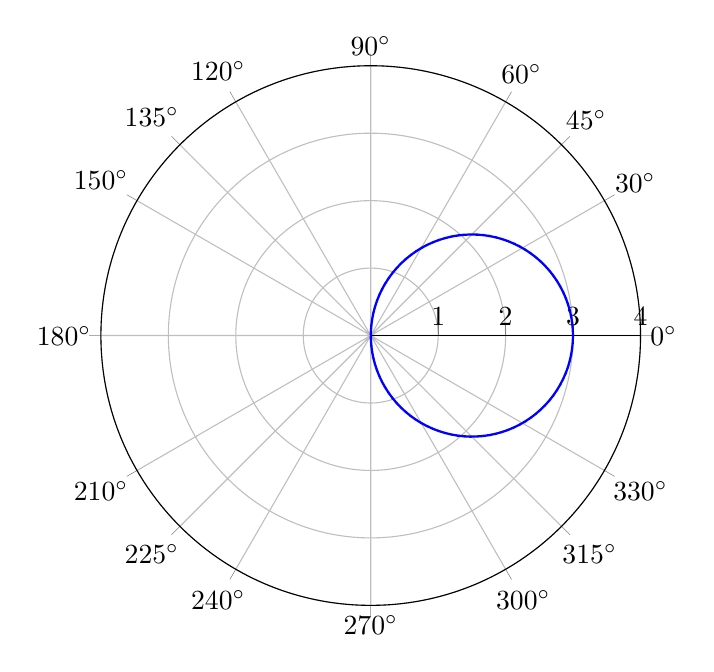
\begin{tikzpicture}
\begin{polaraxis}[
   xticklabel=$\pgfmathprintnumber{\tick}^\circ$,
   xtick={0,30,45,60,90,120,135,150,180,210,225,240,270,300,315,330},
   ytick={1,2,3,4},
   %yticklabel=\empty,
   ymin=0, ymax=4];
   
\addplot[thick, color=blue, domain=0:360, samples=100] {3*cos(x)};  
   

\end{polaraxis}
\end{tikzpicture}
\end{center}

\end{multicols}

\pagebreak

\item $r=-5\sin\theta$

\begin{multicols}{2}
\begin{center}
\begin{tikzpicture}[scale=1]
\begin{axis}[
	axis lines=middle,
	xmin=0, xmax=6.8,
	ymin=-5.25, ymax=5.25,
	xtick={1.570796327,	3.141592654,	4.71238898,	6.283185307},
	ytick={-5,...,5},
	xticklabels={$\frac{\pi}{2}$, $\pi$, $\frac{3\pi}{2}$, $2\pi$},
	axis line style={->},
	%grid=both,
	ticklabel style={font=\tiny,fill=white},
	xlabel=$\theta$, ylabel=$r$,
	xlabel style={at={(ticklabel* cs:1)},anchor=north west},
	ylabel style={at={(ticklabel* cs:1)},anchor=south west}
]

\addplot[thick, samples=100, domain=0:2*pi] {-5*sin(deg(x))};

\end{axis}
\end{tikzpicture}
\end{center}

\columnbreak

\begin{center}
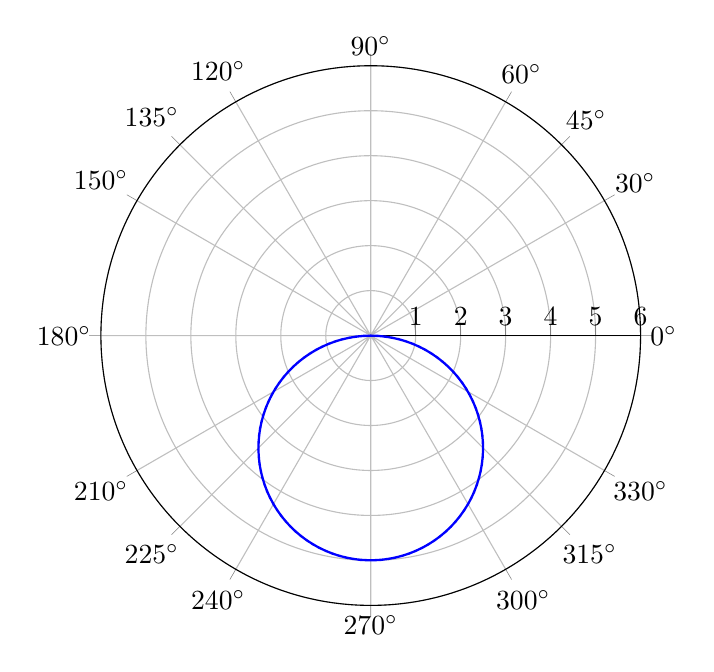
\begin{tikzpicture}
\begin{polaraxis}[
   xticklabel=$\pgfmathprintnumber{\tick}^\circ$,
   xtick={0,30,45,60,90,120,135,150,180,210,225,240,270,300,315,330},
   ytick={1,...,6},
   %yticklabel=\empty,
   ymin=0, ymax=6];
   
\addplot[thick, color=blue, domain=0:360, samples=100] {-5*sin(x)};  
   

\end{polaraxis}
\end{tikzpicture}
\end{center}

\end{multicols}


\item $r=1+5\sin\theta$


\begin{multicols}{2}
\begin{center}
\begin{tikzpicture}[scale=1]
\begin{axis}[
	axis lines=middle,
	xmin=0, xmax=6.8,
	ymin=-4.25, ymax=6.25,
	xtick={1.570796327,	3.141592654,	4.71238898,	6.283185307},
	ytick={-7,...,7},
	xticklabels={$\frac{\pi}{2}$, $\pi$, $\frac{3\pi}{2}$, $2\pi$},
	axis line style={->},
	%grid=both,
	ticklabel style={font=\tiny,fill=white},
	xlabel=$\theta$, ylabel=$r$,
	xlabel style={at={(ticklabel* cs:1)},anchor=north west},
	ylabel style={at={(ticklabel* cs:1)},anchor=south west}
]

\addplot[thick, samples=100, domain=0:2*pi] {1+5*sin(deg(x))};

\end{axis}
\end{tikzpicture}
\end{center}

\columnbreak

\begin{center}
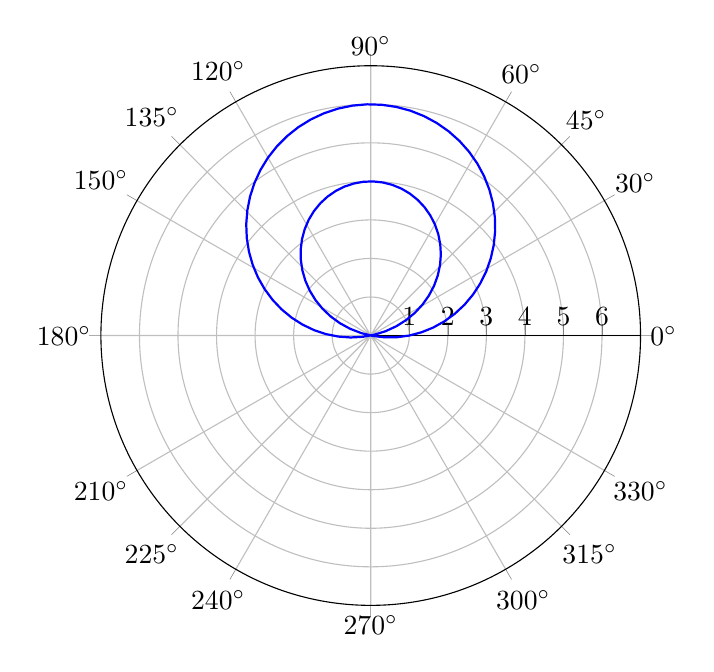
\begin{tikzpicture}
\begin{polaraxis}[
   xticklabel=$\pgfmathprintnumber{\tick}^\circ$,
   xtick={0,30,45,60,90,120,135,150,180,210,225,240,270,300,315,330},
   ytick={1,...,6},
   %yticklabel=\empty,
   ymin=0, ymax=7];
   
\addplot[thick, color=blue, domain=0:360, samples=100] {1+5*sin(x)};  
   

\end{polaraxis}
\end{tikzpicture}
\end{center}

\end{multicols}

\pagebreak

\item $r=2+\sin3\theta$

\begin{multicols}{2}
\begin{center}
\begin{tikzpicture}[scale=1]
\begin{axis}[
	axis lines=middle,
	xmin=0, xmax=6.8,
	ymin=-1.25, ymax=3.25,
	xtick={1.570796327,	3.141592654,	4.71238898,	6.283185307},
	ytick={-7,...,7},
	xticklabels={$\frac{\pi}{2}$, $\pi$, $\frac{3\pi}{2}$, $2\pi$},
	axis line style={->},
	%grid=both,
	ticklabel style={font=\tiny,fill=white},
	xlabel=$\theta$, ylabel=$r$,
	xlabel style={at={(ticklabel* cs:1)},anchor=north west},
	ylabel style={at={(ticklabel* cs:1)},anchor=south west}
]

\addplot[thick, samples=100, domain=0:2*pi] {2+sin(deg(3*x))};

\end{axis}
\end{tikzpicture}
\end{center}

\columnbreak

\begin{center}
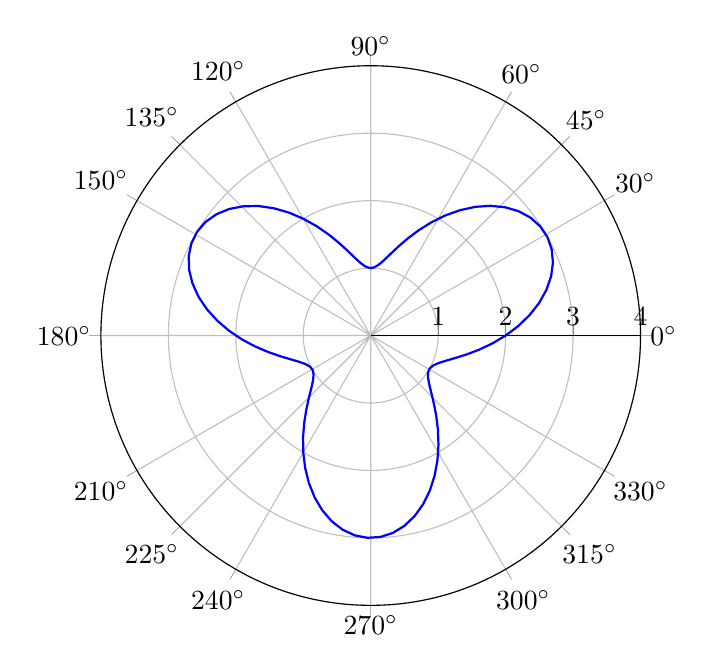
\begin{tikzpicture}
\begin{polaraxis}[
   xticklabel=$\pgfmathprintnumber{\tick}^\circ$,
   xtick={0,30,45,60,90,120,135,150,180,210,225,240,270,300,315,330},
   ytick={1,...,6},
   %yticklabel=\empty,
   ymin=0, ymax=4];
   
\addplot[thick, color=blue, domain=0:360, samples=100] {2+sin(3*x)};  
   

\end{polaraxis}
\end{tikzpicture}
\end{center}

\end{multicols}


\end{enumerate}

\item Find the points on the given curve where the tangent line is horizontal or vertical.

\begin{enumerate}
\item $r=1+\cos\theta$

First we need to calculate $\frac{dx}{d\theta}$ and $\frac{dy}{d\theta}$, but in order to do that, we need to find a function $x$ of $\theta$ and a function $y$ of $\theta$. What equations do we know that relate $x$ and $y$ to $\theta$? The Cartesian representations! We have

\begin{align*}
x&=r\cos\theta=\cos\theta(1+\cos\theta) \\
y&=r\sin\theta=\sin\theta(1+\cos\theta).
\end{align*}

For the horizontal tangents, we examine $\frac{dy}{d\theta}$.

\begin{align*}
\frac{dy}{d\theta}&=(1+\cos\theta)\cos\theta-\sin^2\theta \\
&=2\cos^2\theta+\cos\theta-1 \\
&=(2\cos\theta-1)(\cos\theta+1).
\end{align*}

Now we set these equal to 0.

\begin{multicols}{2}

\begin{align*}
2\cos\theta-1&=0 \\
\cos\theta&=\frac{1}{2} \\
\theta&=\frac{\pi}{3}\text{ or }\frac{5\pi}{3}
\end{align*}

\columnbreak

\begin{align*}
\cos\theta+1&=0 \\
\cos\theta&=-1 \\
\theta&=\pi
\end{align*}

\end{multicols}

So the curve will have horizontal tangents at these values of $\theta$. Plugging these values into our original polar equation gives us the three respective radius values, allowing us to list the three points where the horizontal tangents occur:

\[
\left(\frac{3}{2},\frac{\pi}{3}\right),\hspace{0.25cm}(0,\pi),\hspace{0.25cm}\left(\frac{3}{2},\frac{5\pi}{3}\right)
\]

For the vertical tangents, we examine $\frac{dx}{d\theta}$.

\begin{align*}
\frac{dx}{d\theta}&=-(1+\cos\theta)\sin\theta-\cos\theta\sin\theta \\
&=-\sin\theta(1+2\cos\theta). \\
\end{align*}

Now we set these factors equal to 0.

\begin{multicols}{2}

\begin{align*}
-\sin\theta&=0 \\
\sin\theta&=0 \\
\theta&=0\text{ or }\cancel{\pi}\,^*
\end{align*}

\columnbreak

\begin{align*}
1+2\cos\theta&=0 \\
\cos\theta&=-\frac{1}{2} \\
\theta&=\frac{2\pi}{3}\text{ or }\frac{4\pi}{3}
\end{align*}

\end{multicols}

So the curve will have vertical tangents at these values of $\theta$. Plugging these values into our original polar equation gives us the three respective radius values, allowing us to list the three points where the horizontal tangents occur:

\[
(2,0),\hspace{0.25cm}\left(\frac{1}{2},\frac{2\pi}{3}\right),\hspace{0.25cm}\left(\frac{1}{2},\frac{4\pi}{3}\right)
\]

*Notice that we already determined there was a horizontal tangent at $(0,\pi)$ above. But we got the same point when we tested for a vertical tangent. Which one is it? We test the limit of the ratio of derivatives to check:

\[
\lim_{\theta\rightarrow\pi}\frac{\frac{dy}{d\theta}}{\frac{dx}{d\theta}}=\lim_{\theta\rightarrow\pi}\frac{(2\cos\theta-1)(\cos\theta+1)}{-\sin\theta(1+2\cos\theta)}=0
\]
\vspace{0.5cm}

\item $r=e^\theta$

\begin{align*}
x&=r\cos\theta=e^\theta\cos\theta \\
y&=r\sin\theta=e^\theta\sin\theta.
\end{align*}

\begin{multicols}{2}

\begin{align*}
\frac{dy}{d\theta}&=e^\theta\sin\theta+e^\theta\cos\theta \\
&=e^\theta(\sin\theta+\cos\theta) \\
\end{align*}

\begin{align*}
\sin\theta+\cos\theta&=0 \\
\sin\theta&=-\cos\theta \\
\tan\theta&=-1 \\
\theta&=-\frac{1}{4}\pi+n\pi.
\end{align*}

\columnbreak

\begin{align*}
\frac{dx}{d\theta}&=e^\theta\cos\theta-e^\theta\sin\theta \\
&=e^\theta(\cos\theta-\sin\theta). \\
\end{align*}

\begin{align*}
\cos\theta-\sin\theta&=0 \\
\sin\theta&=\cos\theta \\
\tan\theta&=1 \\
\theta&=\frac{1}{4}\pi+n\pi.
\end{align*}

\end{multicols}

Note that $e^\theta\neq0$ for any $\theta$, so we do not need to consider that factor. Thus, this curve has horizontal tangents at

\[
\left(e^{\pi(n-1/4)},\pi\left(n-\frac{1}{4}\right)\right),
\]

and vertical tangents at

\[
\left(e^{\pi(n+1/4)},\pi\left(n+\frac{1}{4}\right)\right)
\]

\end{enumerate}
\end{enumerate}
\end{document}